\documentclass[a4paper,10pt]{article}
% Requires xelatex

\usepackage{marvosym}
\usepackage{geometry}
\usepackage{fontspec} 					%for loading fonts
\usepackage{xunicode,xltxtra,url,parskip} 	%other packages for formatting
\usepackage{color,graphicx}
\usepackage[usenames,dvipsnames]{xcolor}
\usepackage[big]{layaureo} 				%better formatting of the A4 page
\usepackage{supertabular} 				%for Grades
\usepackage{titlesec}					%custom \section
\usepackage{tikz}
\usepackage{tikzpagenodes}
\usetikzlibrary{calcs}

%Setup hyperref package, and colours for links
\usepackage{hyperref}
\definecolor{linkcolour}{rgb}{0,0.2,0.6}
\hypersetup{colorlinks,breaklinks,urlcolor=linkcolour, linkcolor=linkcolour}

%FONTS
\defaultfontfeatures{Mapping=tex-text}
\setmainfont{Fontin}[
SmallCapsFont = *-SmallCaps,
BoldFont = *-Bold,
ItalicFont = *-Italic
]

% setup skill bars
\usepackage{xcolor}
\definecolor{noskillgray}{gray}{0.8}
\definecolor{skilledblack}{rgb}{0.1,0.1,0.1}

\makeatletter
\newdimen\skillb@level
\newdimen\skillb@length
\newdimen\skillb@height
\skillb@length=80pt%
\skillb@height=5pt%
\newcommand*{\skillbar}[1]{%
    \skillb@level=\dimexpr#1\skillb@length/100\relax%
    {\color{skilledblack}\rule{\skillb@level}{\skillb@height}}%
    {\color{noskillgray}%
        \rule{\dimexpr\skillb@length-\skillb@level\relax}{\skillb@height}}%
}
\newcommand*{\skill}[2]{%
	\par\noindent%
    {\hskip 1ex\textsc #1}\hspace{10pt}\skillbar{#2}%
}
\makeatother

%%%

\titleformat{\section}{\Large\scshape\raggedright}{}{0em}{}[\titlerule]
\titlespacing{\section}{0pt}{3pt}{10pt}
\titleformat{\subsection}{\large\scshape\centering}{}{0em}{}
\titlespacing{\subsection}{0pt}{3pt}{8pt}
\titlespac

% -------------------------------------------------------
% USER DEFINED SETTINGS
% -------------------------------------------------------
\newcommand{\email}[1]{\href{mailto:#1}{#1}}

%--------------------BEGIN DOCUMENT----------------------
\begin{document}

\pagestyle{empty} % non-numbered pages

\font\fb=''[cmr10]'' %for use with \LaTeX command

%--------------------TITLE-------------

\begin{tikzpicture}[remember picture,overlay]
	\clip (12, -1.25)
	  circle (1.5cm) node {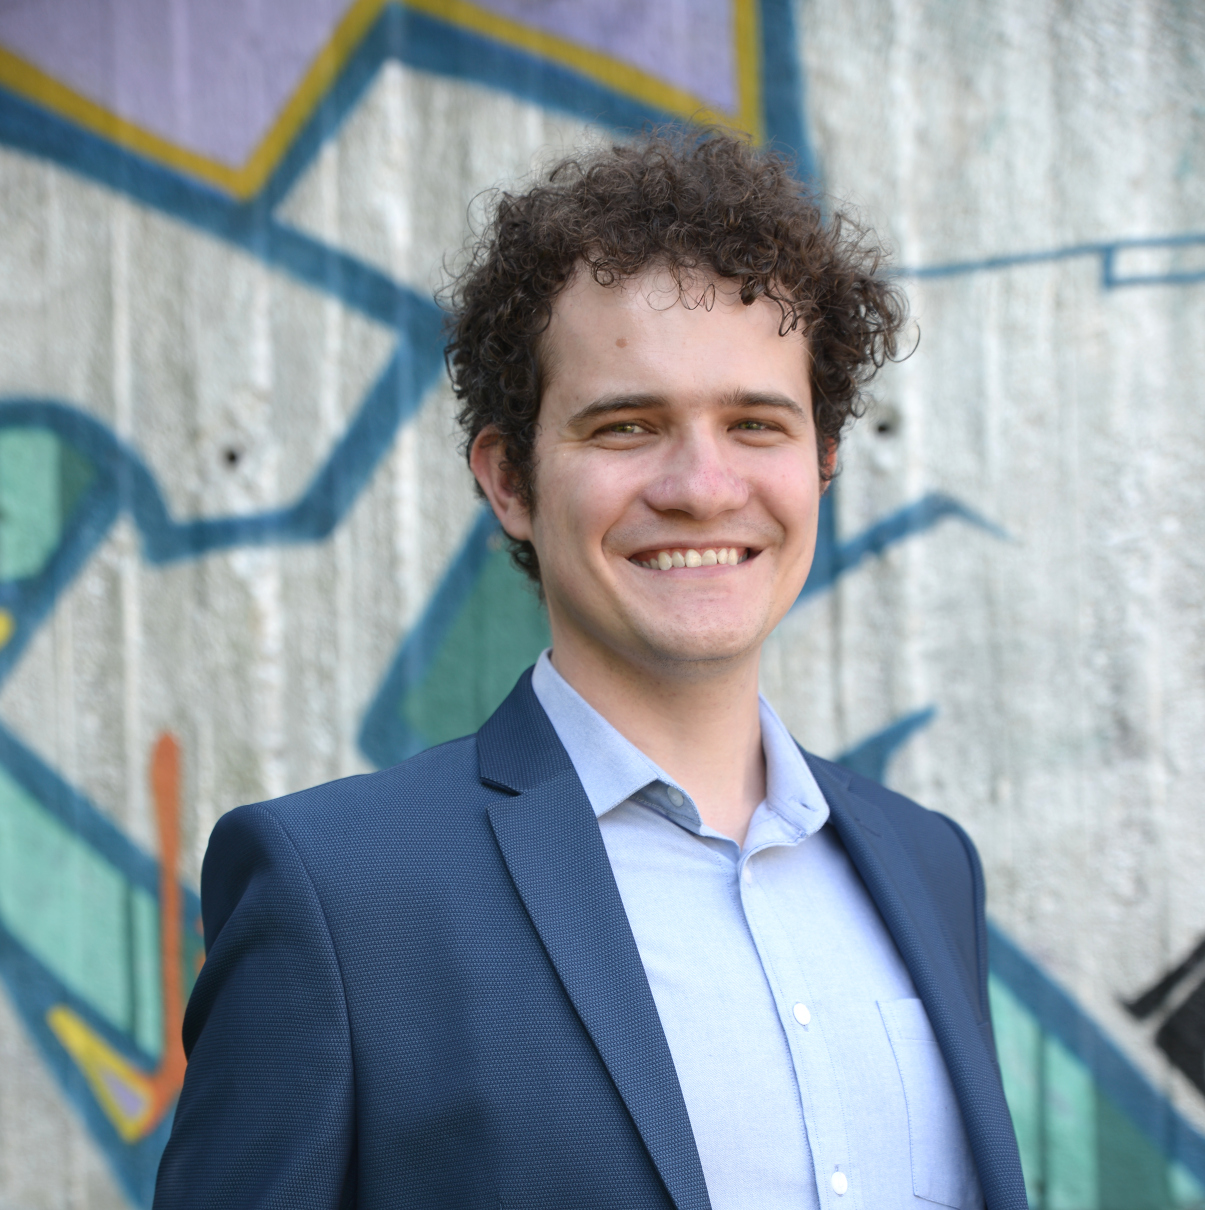
\includegraphics[width=3cm]{profile.JPG}};
\end{tikzpicture}

\par{\raggedright
		{\hskip 1cm\Huge Jason \textsc{Webster}
	}\bigskip\par}

\begin{left}
	\begin{tabular}{rl}
		\textsc{LinkedIn:} & \href{https://www.linkedin.com/in/jasonrobwebster/}{linkedin.com/in/jasonrobwebster/} \\
		\textsc{GitHub:} & \href{https://github.com/jasonrobwebster/}{github.com/jasonrobwebster/}
	\end{tabular}
\end{left}



%--------------------SECTIONS-----------------------------------
\section{Personal}

\begin{tabular}{rl}
	\textsc{Address:} & 84 Marais Avenue                                                    \\
%	                  & Klein Welgevonden Drive                                            \\
	                  & Pretoria                                                       \\
	                  & 0157                                                               \\
	                  & South Africa                                                       \\
	  \textsc{Phone:} & +27 79 393 0971                                                    \\
	  \textsc{email:} & \email{jasonrobwebster@gmail.com}
\end{tabular}
\section{Languages}

\begin{tabular}{rl}
	  \textsc{English:} & Mother tongue   \\
	\textsc{Afrikaans:} & Basic Knowledge 
\end{tabular}
\section{Skills}

% \subsection{Analysis}
% \begin{center}
% 	\begin{supertabular}{rlrl}
% 		Modelling & \skillbar{95} & Excel & \skillbar{90} \\
% 		Mathematica & \skillbar{85} & SQL & \skillbar{85} \\
% 		Tensorflow & \skillbar{85} & Pytorch & \skillbar{85} \\
% 		Flask & \skillbar{80} & HTML & \skillbar{80} \\
% 		GDScript & \skillbar{80} & CSS & \skillbar{70} \\
% 		C\# & \skillbar{55} & JavaScript & \skillbar{40} \\
% 		ActionScript & \skillbar{40} & C++ & \skillbar{40} \\
% 		C & \skillbar{35} & Java & \skillbar{30} \\
% 	\end{supertabular}
% \end{center}

% \subsection{Software}
% \begin{center}
% 	\begin{supertabular}{rlrl}
% 		Python & \skillbar{95} & Matlab & \skillbar{90} \\
% 		Mathematica & \skillbar{85} & SQL & \skillbar{85} \\
% 		Tensorflow & \skillbar{85} & Pytorch & \skillbar{85} \\
% 		Flask & \skillbar{80} & HTML & \skillbar{80} \\
% 		GDScript & \skillbar{80} & CSS & \skillbar{70} \\
% 		C\# & \skillbar{55} & JavaScript & \skillbar{40} \\
% 		ActionScript & \skillbar{40} & C++ & \skillbar{40} \\
% 		C & \skillbar{35} & Java & \skillbar{30} \\
% 	\end{supertabular}
% \end{center}

\begin{supertabular}{p{1.8cm}|p{12cm}}
	\textsc{Software}  & Expert: Python \\
					   & Experienced: AWS, Matlab, Mathematica, GDScript, \LaTeX{}, SQL             \\
	                   & Novice: ActionScript, Delphi, C, C\#, JavaScript, MongoDB                  \\
	\multicolumn{2}{c}{} \\
	\textsc{Research}  & Optics, Electron Microscopy, Statistical Mechanics, Wave Propagation and Dynamics, Natural Language Processing, Machine Learning \\
	\multicolumn{2}{c}{} \\
	\textsc{Soft}	   & Writing, Communicating, Public Speaking, Presenting \\
	\multicolumn{2}{c}{} \\
	\textsc{Technical} & Laser Design and Construction, Laser Operation, Cloud Computing \\
	\multicolumn{2}{c}{} \\
	\textsc{Web}	   & Experienced: Alembic, Flask, Jinja, HTML \\
					   & Novice: Django, CSS \\
\end{supertabular}

\section{Work Experience}

\begin{supertabular}{l|p{11cm}}
	\textsc{Jan 2019 -}  		& Junior Data Scientist at \textsc{Explore-AI} \\
	\textsc{Present}			& \emph{Teaching and Consulting} \\
								& \footnotesize{Course facilitator for 100 data science students in Johannesburg. Designed and implemented curriculum for online courses. Supervised 4 teams of interns positioned at and consulting with a multitude of different companies. Organized a monthly meetup event (see Leadership). Currently launching a research division within the company.} \\
	%\textsc{Jan 2017 -}  		& Private Tutor at \textsc{First Tutors} \\
	%\textsc{Dec 2018}			& \emph{Mathematics and Physics Tutoring} \\
	%							& \footnotesize{Provided private mathematics and physics tutoring to a number of students in multiple fields. } \\
	%\multicolumn{2}{c}{} \\
	%\textsc{Jan - Dec 2016} 	& 2\textsuperscript{nd} year Tutor for the \textsc{University of the Witwatersrand} \\
	%							& \emph{Classical Mechanics and Electrodynamics} \\
	%							& \footnotesize{Was tasked with giving tutorial sessions and marking student scripts for the 2\textsuperscript{nd} year Physics Major students. Learned to teach in front of a large crowd.} \\
	\multicolumn{2}{c}{} \\
	\textsc{Jun - Jul 2016}    	& Research Collaborator at \textsc{University of Oregon} \\
	 							& \emph{Reference:} Dr.\ Ben McMorran | \email{mcmorran@uoregon.edu}\\
	 							& \footnotesize{Developed new methods of generating electron vortex beams, and was trained to operate a transmission electron microscope. Helped form new collaborations between my research group and that of Ben McMorran’s.}\\
	\multicolumn{2}{c}{} \\
	\textsc{Dec 2015 --} 		& Intern at the \textsc{National Institute for Theoretical Physics (NITheP)} \\
	\textsc{Jan 2016} 			& \emph{Reference:} Prof.\ Michael Kastner | \email{kastner@sun.ac.za}\\
	 							& \footnotesize{Studied a long-range highly constrained spin model that has shown equivalence to certain Bose-Einstein condensates. Learned to tackle extremely technical and challenging theoretical problems, and learned a great deal of quantum mechanics and statistical physics in the process.}\\
	\multicolumn{2}{c}{} \\
	\textsc{Jul 2012 --} 		& Intern at the \textsc{Council for Scientific and Industrial Research (CSIR)} \\
	\textsc{Dec 2014}			& \emph{Reference:} Dr.\ Hermann Uys | \email{hermann@sun.ac.za}\\
	 							& \footnotesize{Interned throughout various summer and winter vacations. Was tasked with a number of projects, including: building a large-scale ion trap for use in public demonstrations, simulating the motion of trapped ions, and investigating rotational broadening effects on molecular spectra.} \\
\end{supertabular}
\section{Projects}

\begin{supertabular}{p{1.8cm}|p{12cm}}
	\textsc{Mar 2020} & ASSA Covid Model \\
	& \small\emph{Work Related Project -- Technical Lead}\href{https://github.com/Percept-Health-Solve/seir-model}{\hfill| \footnotesize{Github Link}}\\
	& \footnotesize{Mathematically modelled, built, and maintained the Acturial Society of South Africa's (ASSA's) Covid-19 model. This is an epidemiological model that is built to predict the number of infections, hospitalisations, icu usage, and deaths due to the Covid-19 pandemic in South Africa. The algorithm is built to operate at a national level, as well as a provincial level. This model was a culmination of a team effort of over 20 volunteer actuaries from multiple organisations.} \\
	\multicolumn{2}{c}{} \\
	\textsc{Jan 2019} & Self-driving Car and GamePy \\
	& \small\emph{Personal Project}\href{https://github.com/jasonrobwebster/gamepy}{\hfill| \footnotesize{Github Link}}\\
	& \footnotesize{I built a simulated self-driving car in the game "Burnout: Ultimate Paradise". I gathered data by recording myself playing the game and used this to train a convolutional neural network that mapped images to keystrokes. I managed to make this work using local hardware while being tightly constrained by my budget and GPU size. The result of this project was a general-purpose package dubbed "gamepy" that allows one to record themselves and their keystrokes while acting in a simulated environment. It also allows integration to the game environment to be able to then "play" the game using a prediction of the model. I wrote about my experiences building this in a blog post for OfferZen and can be read \href{https://www.offerzen.com/blog/how-to-develop-a-self-driving-car-in-under-a-week}{here}.} \\
	\multicolumn{2}{c}{} \\
	\textsc{Jun 2018} & AlphaZero Clone \\
	& \small\emph{Personal Project}\href{https://github.com/jasonrobwebster/alphazero-clone}{\hfill| \footnotesize{Github Link}}\\
	& \footnotesize{A clone of the alpha zero algorithm, written entirely by me. The algorithm was used by Google's Deepmind to beat the world's best Go player, as well as the best Chess engine (stockfish). The algorithm learns to play any perfect information board game entirely through self-play and reinforcement learning.} \\
	\multicolumn{2}{c}{} \\
	% \textsc{Mar 2018} & AtomPy \\
	% & \emph{Study Project}\href{https://github.com/jasonrobwebster/atompy}{\hfill| \footnotesize{Github Link}} \\
	% & \footnotesize{I attempted to build a symbolic package for modelling and deriving the equations of motion for an atomic system using Python. I first built the symbolic package from scratch, but later used SymPy as my backend. I managed to get as far as deriving the equations of motion for simple atomic systems, but ended up abandoning the project as it could not handle larger, more complex systems. Note this project is not well documented as it has been abandoned.} \\
	% \multicolumn{2}{c}{} \\
	\textsc{Nov 2017} & Variational Autoencoder \\
	& \small\emph{Personal Project}\href{https://github.com/jasonrobwebster/vae-keras-pytorch}{\hfill| \footnotesize{Github Link}}\\
	& \footnotesize{Variational autoencoders (VAEs) are a neural network architecture that represent high dimensional data (e.g. images) in a low dimensional latent space. This is similar to principle component analysis, however, what makes a VAE different is that it learns the parameters of a probability distribution for each data point, allowing for the generation of new data points. I worked on duplicating this architecture at home, and can now implement a VAE, PixelVAE, and VQ-VAE in tensorflow and keras. The github link shows an example of a simple VAE.} \\
\end{supertabular}
\section{Education}

\begin{supertabular}{rl}
	\textsc{Dec} 2018 & Master of Science in \textsc{Physics}, \textbf{Stellenbosch University}                                                 \\
					  & \small\emph{With distinction}, \emph{Summa cum laude} \\
					  & Thesis: ``Towards Atomic Physics Using Spatially Structured Light''                                                     \\
	                  & \small Advisor: Dr. Hermann Uys                                                                                       \\
	                  &                                                                                                                         \\
	                  & \\ % filler
	                  & \\ %filler
	\textsc{Mar} 2016 & BSc Honours in  \textsc{Physics}, \textbf{University of the Witwatersrand}                                              \\
	                  & \small\emph{With distinction}, \emph{Summa cum laude}                                                                  \\
	                  & Thesis: ``Electron Vortex Beams and Non-Radiating Accelerating Electrons''                                            \\
	                  & \small Advisor: Prof. Andrew Forbes                                                                                     \\
	                  & \normalsize \textsc{Average}: 91.1\% | \textsc{Gpa} 3.92/4 \hyperlink{honours}{\hfill| \footnotesize Academic Record}  \\
	                  &                                                                                                                         \\
	\textsc{Mar} 2015 & BSc in \textsc{Physics} and \textsc{Applied Mathematics}, \textbf{University of the Witwatersrand}                      \\
	                  & \small\emph{With distinction}, \emph{Summa cum laude}                                                                  \\
	                  & \normalsize \textsc{Average}: 85.0\% | \textsc{Gpa} 3.84/4 \hyperlink{undergrad}{\hfill| \footnotesize Academic Record} \\
	                  &                                                                                                                         \\
	\textsc{Dec} 2012 & Highschool Certificate, \textbf{Curro Bankenveld} \\
\end{supertabular}
\section{Notable Awards}

\begin{supertabular}{p{1.8cm}|p{12cm}}
	\textsc{Dec 2018} & S2A3 Medal, \textbf{Stellenbosch University} \\
	& \small{Awarded to the top MSc graduate in the natural sciences at Stellenbosch University.} \\
	\multicolumn{2}{c}{} \\
	\textsc{Dec 2016} & Chancellor's Medal, \textbf{University of the Witwatersrand} \\
	& \small{Awarded to the top overall graduating student across all fields of study at the university. Presented by Adam Habib, then Vice Chancellor of Wits.} \\
	\multicolumn{2}{c}{} \\
	\textsc{Mar 2016} & Samuel Goodman Memorial Medal, \textbf{University of the Witwatersrand} \\
	& \small{Awarded to the most distinguished Honours graduate across the Faculty of Science.} \\
	\multicolumn{2}{c}{} \\
	\textsc{Mar 2016} & Jan Loubser Medal, \textbf{University of the Witwatersrand} \\
	& \small{Awarded to the most distinguished Honours graduate across the Faculty of Science.} \\
	\multicolumn{2}{c}{} \\
	\textsc{Mar 2016} & Element Six Diamond Research Lab and DST/NRF Centre of Excellence in Strong Materials Medal, \textbf{University of the Witwatersrand} \\
	& \small{Awarded for outstanding performance in the Honours year of study in Physics.} \\
	\multicolumn{2}{c}{} \\
	\textsc{Dec 2015} & William Cullen Medal, \textbf{University of the Witwatersrand} \\
	& \small{Awarded to the most distinguished Bachelor of Science graduand in the Faculty of Science.} \\
	\multicolumn{2}{c}{} \\
	% \textsc{Dec 2015} & Element Six Diamond Research Lab and DST/NRF Centre of Excellence in Strong Materials Medal, \textbf{University of the Witwatersrand} \\
	% & \small{Awarded for outstanding performance in Physics III.} \\
\end{supertabular}

\section{Publications}

\begin{supertabular}{p{1.8cm}|p{12cm}}
	\textsc{May 2020} & Neural machine translation for South Africa's official languages \\
	& \small{L Martinus, \textbf{J Webster}, J Moonsamy, M Shaba, R Moosa, R Fairon, \emph{Workshop paper at AfricaNLP, ICLR 2020}} \\
	& \footnotesize{Calculated a benchmark translation score for all of South Africa's official languages using state of the art neural machine translation techniques. These were the first such scores published at the time.} \\
	\multicolumn{2}{c}{} \\
	\textsc{Apr 2019} & Coiling free electron matter waves \\
	& \small{J Pierce, \textbf{J Webster}, H Larocque, E Karimi, B McMorran, A Forbes, \emph{New Journal of Physics 21 (4), 043018}} \\
	& \footnotesize{Demonstrated the construction of a novel class of angularly accelerating electron beams. Provided the means to construct the beam, while my collaborators performed the experiment. Contributed to the theoretical analysis of the electromagnetic field during the electron’s propagation. This paper was based on work from my Honours thesis.} \\
	\multicolumn{2}{c}{} \\
	\textsc{Jun 2018} & Subexponentially Growing Hilbert Spaces and Nonconcentrating Distributions in a Constrained Spin Model \\
	& \small{\textbf{J Webster}, M Kastner, \emph{Journal of Statistical Physics 171.3 (2018): 449-461}} \\
	& \footnotesize{Studied a highly constrained long-range spin model for use in a specially prepared Bose-Einstein condensate experiment. Resulted from the work done during my internship at NITheP.} \\
	\multicolumn{2}{c}{} \\
	\textsc{Jan 2017} & Radially dependant angular acceleration of twisted light \\
	& \small{\textbf{J Webster}, C Rosales-Guzm\'an, A Forbes, \emph{Optics letters 42.4 (2017): 675-678}} \\
	& \footnotesize{Developed a new technique of controlling the angular acceleration of laser light by using the Guoy phase in Laguerre-Gauss beams. This paper was featured as one of the top downloads on OSA’s website during February 2017.} \\
\end{supertabular}
\section{Conferences}

\begin{tabular}{p{1.8cm}|p{12cm}}
	\textsc{Sep} 2019 & Deep Learning Indaba 2019 \\
	& \textbf{Nairobi, Kenya} \\
	& \small{Poster: ``On VAE Approximation Errors''\href{https://drive.google.com/file/d/1V9z54ngcrdxrn5kBbgTzPTeNhwfJBX-n/view?usp=sharing}{\hfill| Poster Link}} \\
	\multicolumn{2}{c}{} \\
	\textsc{Sep} 2018 & Deep Learning Indaba 2018 \\
	& \textbf{Stellenbosch, South Africa} \\
	\multicolumn{2}{c}{} \\
	\textsc{Sep} 2017 & International Conference on Optical Angular Momentum \\
	& \textbf{Anacapri, Italy} \\
	& \small{Poster: ``Angularly Accelerating Electron Waves''} \\
	\multicolumn{2}{c}{} \\
	\textsc{Jul} 2017 & SAIP 62\textsuperscript{nd} Annual Conference \\
	& \textbf{Stellenbosch, South Africa} \\
	& \small{Presentation: ``Nano-fabricated Si3N4 holograms for probing matter with structured waves.'' | Awarded best Honours presentation in the Material Sciences Division.} \\
	& \small{Presentation: ``Non-radiating accelerating electrons?''}
\end{tabular}
\section{Leadership}

\begin{supertabular}{p{1.8cm}|p{12cm}}
	\textsc{Jun 2019 --} & Explore-AI Meetup Organizer\\
	\textsc{Mar 2020}& \small{Started, organized, and maintained a meetup group for the public. Organized speakers for the event. More details can be found at \href{https://www.meetup.com/Explore-AI-JHB-Meetup-Group/}{https://www.meetup.com/Explore-AI-JHB-Meetup-Group/}} \\
	\multicolumn{2}{c}{} \\
	\textsc{Jan 2018} & Chris Engelbrecht Summer School Organisational Committee \\
	& \small{Served as head of accommodation management. Ensured that a local python package repository was accessible to the attendees. Assisted in the set up of the venue.} \\
	\multicolumn{2}{c}{} \\
	\textsc{Jan 2017 --} & Stellenbosch OSA Student Chapter Committee \\
	\textsc{Dec 2017} & \small{Head of media in the student chapter organisational committee. Was placed in charge of designing posters/flyers for events. Designed a website for the committee.} \\
\end{supertabular}
\section{Committees and Societies}

\begin{tabular}{lp{12cm}}
	2017 & Maties Underwater Club \\
	& \small{Member of the Stellenbosch University scuba diving club.} \\
	& \\
	2015 - & Wits Astronomy Club \\
	2016& \small{Member of the Wits University Astronomy Club. I've always had a passion for astronomy, and had briefly considered becoming an Astrophysicist at one stage in my life.} \\
	& \\
	2016 - & OSA Student Chapter Member \\
	2018 & \small{Maintained participation in outreach activities to local schools.} \\
	& \\
	2014 - & International Golden Key Society \\
	\textsc{present} & \small{Invited due to the academic success in my 1\textsuperscript{st} year of undergraduate studies.}
\end{tabular}
\section{Certificates}

\begin{supertabular}{p{1.8cm}|p{12cm}}
	\textsc{Apr} 2018 & NMISA Basic Laser Safety Course \\
	\multicolumn{2}{c}{} \\
	\textsc{May} 2017 & Writing for Peer Review
\end{supertabular}
\section{Personal Achievements}

\begin{supertabular}{p{1.8cm}|p{12cm}}
	2018 & Modelled a self-driving car using deep learning \\
	& \footnotesize{Built a self-driving car using a deep learning model, trained on recorded footage of myself playing “Burnout: Ultimate Paradise”.  Learned about convolutional neural networks, GPU memory management, and working in a simulated environment. An article on this project can be found at \href{https://www.offerzen.com/blog/how-to-develop-a-self-driving-car-in-under-a-week}{offerzen.com/blog/how-to-develop-a-self-driving-car-in-under-a-week}}. \\
	\multicolumn{2}{c}{} \\
	2016 & Graduated from Wits University as one of the top performing students across all fields of study \\
	& \footnotesize{Received the highest academic honour, the Chancellor’s medal, for my academic performance at Wits.} \\
	\multicolumn{2}{c}{} \\
	2015 & Became a ``professional'' game developer \\
	& \footnotesize{I developed a small web-based game using the ActionScript programming language, and received a pay cheque of \$25 in advertising revenue from the website that hosted it.}\\
\end{supertabular}
\section{Interests and Hobbies}

Technology, Programming, Deep Learning, Machine Learning, Computer Vision, Reinforcement Learning \\
Physics, Optics, Quantum Mechanics, Quantum Field Theory, Astronomy \\
Art, Game Design, Digital Painting, 3D Rendering and Animation

\newpage
\par{\centering \huge Academic Record\par}

\bigskip
\hrule
\bigskip

\par{\centering\Large \hypertarget{honours}{BSc Honours in \textsc{Physics}}\par}
{\centering \textbf{University of the Witwatersrand}\par}\normalsize
\begin{center}
	\begin{tabular}{lccc}
	\multicolumn{1}{c}{\textsc{Course}} & \textsc{Credits} & \textsc{Mark} & \textsc{US Code}\\ \hline
	Quantum Mechanics & 13 & 100 & A \\
	Statistical Physics & 13 & 72 & B+ \\
	Nuclear Physics & 13 & 75 & A \\
	Electrodynamics & 13 & 99 & A \\
	Solid State Physics & 13 & 91 & A \\
	General Relativity & 13 & 96 & A \\
	Introduction to Quantum Field Theory & 13 & 96 & A \\
	Research Project & 30 & 95 & A \\
	\cline{2-4}
	& & \textsc{Ave} & 91.1  \\
	& & \textsc{Gpa} & 3.92 
	\end{tabular}
\end{center}

\bigskip
\hrule
\bigskip

\par{\centering\Large \hypertarget{undergrad}{Undergraduate BSc \textsc{Physics} and \textsc{Applied Mathematics}}\par}
{\centering \textbf{University of the Witwatersrand}\par}\normalsize

\begin{center}

	\tablefirsthead{%
	  \multicolumn{1}{c}{Course} & \textsc{Credits} & \textsc{Mark} & \textsc{US Code}\\ \hline
	}
	\tablehead{%
	\multicolumn{1}{c}{Course} & \textsc{Credits} & \textsc{Mark} & \textsc{US Code}\\ \hline
	}
	\tabletail{%
	}
	\tablelasttail{}	
	
	 \begin{supertabular}{lccc}
	 Computational and Applied Mathematics I & 36 & 77 & A \\
	 Computer Science I & 36 & 94 & A \\
	 Algebra I & 15 & 72 & B+ \\
	 Calculus I & 21 & 85 & A \\
	 Physics I (Major) & 36 & 87 & A \\
	 Computational and Applied Mathematics II & 48 & 93 & A \\
	 Basic Analysis II & 16 & 71 & B+ \\
	 Differential Equations II & 8 & 77 & A \\
	 Multivariable Calculus II & 24 & 56 & C \\
	 Advanced Analysis II & 8 & 92 & A \\
	 Group Theory II & 8 & 85 & A \\
	 Linear Algebra II & 8 & 83 & A \\
	 Physics IIA (Major) & 24 & 78 & A \\
	 Physics IIB (Major) & 24 & 86 & A \\
	 Computational and Applied Mathematics III & 48 & 93 & A \\
	 Quantum Mechanics III & 11 & 96 & A \\
	 Quantum Mechanics and its Applications & 11 & 100 & A \\
	 Statistical Physics III & 11 & 90 & A \\
	 Waves and Modern Optics & 11 & 90 & A \\
	 Advanced Experimental Physics and Project & 28 & 86 & A \\
	 \cline{2-4}
	 & & \textsc{Ave} & 85.0  \\
	 & & \textsc{Gpa} & 3.84
	 \end{supertabular}
\end{center}
%\bigskip
%\hrule
%\bigskip

\end{document}
